\subsection{Coffman conditions}\label{coffman-conditions}

There are four \emph{necessary} and \emph{sufficient} conditions for
deadlock. These are known as the Coffman conditions.

\begin{itemize}
\itemsep1pt\parskip0pt\parsep0pt
\item
  Mutual Exclusion
\item
  Circular Wait
\item
  Hold and Wait
\item
  No pre-emption
\end{itemize}

All of these conditions are required for deadlock, so let's discuss each
one in turn. First the easy ones-

\begin{itemize}
\itemsep1pt\parskip0pt\parsep0pt
\item
  Mutual Exclusion: The resource cannot be shared
\item
  Circular Wait: There exists a cycle in the Resource Allocation Graph.
  There exists a set of processes \{P1,P2,\ldots{}\} such that P1 is
  waiting for resources held by P2, which is waiting for P3,\ldots{},
  which is waiting for P1.
\item
  Hold and Wait: A process acquires an incomplete set of resources and
  holds onto them while waiting for the other resources.
\item
  No pre-emption: Once a process has acquired a resource, the resource
  cannot be taken away from a process and the process will not
  voluntarily give up a resource.
\end{itemize}

\subsection{Examples}\label{examples}

Two students need a pen and paper:

\begin{itemize}
\itemsep1pt\parskip0pt\parsep0pt
\item
  The students share a pen and paper. Deadlock is avoided because Mutual
  Exclusion was not required.
\item
  The students both agree to grab the pen before grabbing the paper.
  Deadlock is avoided because there cannot be a circular wait.
\item
  The students grab both the pen and paper in one operation (``Get both
  or get none''). Deadlock is avoided because there is no \emph{Hold and
  Wait}
\item
  The students are friends and will ask each other to give up a held
  resource. Deadlock is avoided because pre-emption is allowed.
\end{itemize}

\subsection{Livelock}\label{livelock}

Livelock is \emph{not} deadlock-

Consider the following `solution'

\begin{itemize}
\itemsep1pt\parskip0pt\parsep0pt
\item
  The students will put down one held resource if they are unable to
  pick up the other resource within 10 seconds. This solution avoids
  deadlock however it may suffer from livelock.
\end{itemize}

Livelock occurs when a process continues to execute but is unable to
make progress.\\In practice Livelock may occur because the programmer
has taken steps to avoid deadlock. In the above example, in a busy
system, the student will continually release the first resource because
they are never able to obtain the second resource. The system is not
deadlock (the student process is still executing) however it's not
making any progress either.

\subsection{Dining Philosophers}\label{dining-philosophers}

The Dining Philosophers problem is a classic synchronization problem.
Imagine I invite N (let's say 5) philosophers to a meal. We will sit
them at a table with 5 chopsticks (one between each philosopher). A
philosopher alternates between wanting to eat or think. To eat the
philosopher must pick up the two chopsticks either side of their
position (the original problem required each philosopher to have two
forks). However these chopsticks are shared with his neighbor.

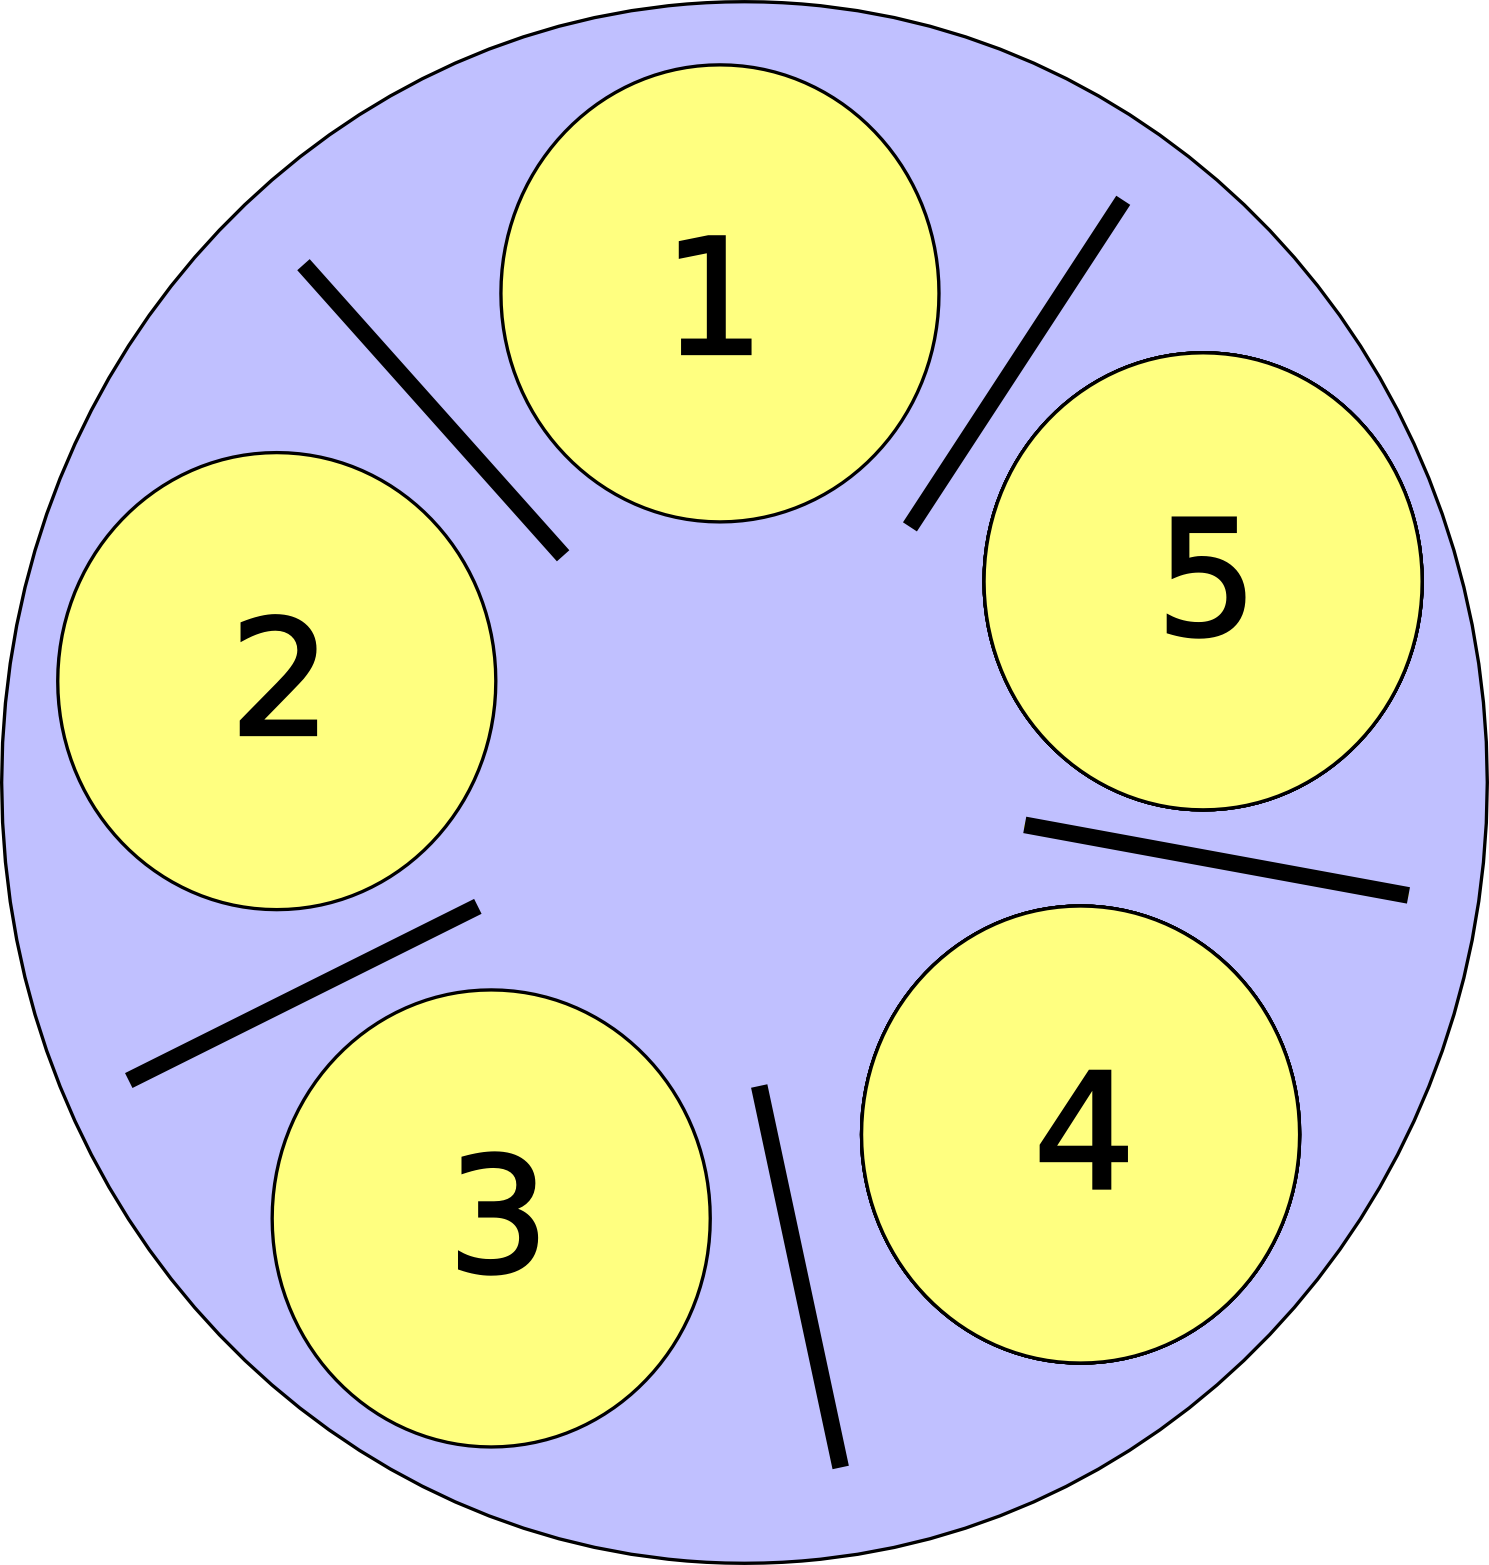
\includegraphics{https://raw.githubusercontent.com/wiki/angrave/SystemProgramming/5DiningPhilosophers.png}

Is is possible to design an efficient solution such that all
philosophers get to eat? Or, will some philosophers starve, never
obtaining a second chopstick? Or will all of them deadlock? For example,
imagine each guest picks up the chopstick on their left and then waits
for the chopstick on their right to be free. Oops - our philosophers
have deadlocked!
